%!TEX root = ../index.tex

% 
% Related work
% 

\section{Related Work}

In this section, we address the state of the art of the research topics, more relevant to our proposed work, namely: Cloud Computing, Volunteer Computing, P2P Networks and the Web Platform.

% 
%---------{Cloud computing and Open Source Cloud Platforms}-------
% 
\subsection{Cloud computing and Open Source Cloud Platforms}

Cloud Computing is a term used to describe a large number of computers, connected through a network. The computing power from these computers is typically made available as virtual machines, without a real physical existence, enabling the possibility to scale up and down its resources on the fly, without affecting the end user.

Cloud Computing today is available as a set of Services, from Infrastructure(IaaS), Platform (PaaS), Software (SaaS), Network (NaaS) and physical hardware (Metal as a Service). However, the idea of having computing organized as a public utility just like the telephone or the electricity service is not new, it was envisioned around 1961, by Professor John McCarthy, who said in MIT's centennial celebration:

  \textit{``Computing may someday be organized as a public utility just as the telephone system is a public utility, Each subscriber needs to pay only for the capacity he actually uses, but he has access to all programming languages characteristic of a very large system. Certain subscribers might offer service to other subscribers. The computer utility could become the basis of a new and important industry.''}, Professor John McCarthy.

Cloud computing presents several advantages comparing to the Conventional Data Center type of architecture\cite{Armbrust}, seen in Table~\ref{tab:advantagesofcloudcomputing}, but there are some tradeoffs such as the `lock-in' syndrome, which locks the platforms to a specific cloud provider due to lack of interoperability and portability of the software stack, plus there is currently also security issues because of the shared CPU and physical memory between different applications from different clients, which enables one of the clients to access data from the other if the application is not well confined.

\begin{table}
  \begin{tabular}{ c | c | c }
  \hline \\
  Advantage & Public Cloud & Conventional Data Center \\
  \hline \\
  Appearance of infinite computing resources on demand & Yes & No \\
  \hline \\
  Elimination of an up-front commitment by Cloud users & Yes & No \\
  \hline \\
  Ability to pay for use of computing resources on a short-term basis as needed & Yes & No \\
  \hline \\
  Economies of scale due to very large data centers & Yes & Usually not \\
  \hline \\
  Higher utilization by multiplexing of workloads from different organizations & Yes & Depends on company size \\
  \hline \\
  Simplify operation and increase utilization via resource virtualizations & Yes & No \\
  \hline  
  \end{tabular}
  \caption{Comparing public clouds and private data centers.}
  \label{tbl:advantagesofcloudcomputing}
\end{table}

\subsubsection{Cloud interoperability}

The lack of portability was identified as a major problem by growing companies and become one of the main factors when opting for a Cloud Provider, the industry realized this issue and started what is known as OpenStack\footnote{http://www.openstack.org/}.

OpenStack is an ubiquitous open source cloud computing platform for public and private clouds. It was founded by Rackspace Hosting and NASA, OpenStack has grown to be a standard of massively scalable open source cloud operating system. The main goal is go give the opportunity to any company to create their cloud stack and therefore, be compatible with other cloud providers since day one. All OpenStack software is licensed under the Apache 2.0 license, giving the possibility for anyone to involve the project and contribute. 

Although OpenStack is free and open source, there is an underlying lie that is the fact that you still have to use OpenStack in order to have portability, it is a more generalized version of the `lock-in syndrome'. We have currently other solutions available that give application developer an abstraction on top of different Cloud Providers, instead of changing the architecture of each Cloud, such as: IEEE Intercloud\footnode{http://cloudcomputing.ieee.org/intercloud}, pkgcloud\footnote{https://github.com/nodejitsu/pkgcloud} and Eucalyptus\cite{Nurmi2009}, described in the following two paragraphs.


\paragraph{\textbf{IEEE Intercloud -}} % (fold)
\label{par:IEEE Intercloud }

% paragraph IEEE Intercloud - (end)


\paragraph{\textbf{pkgcloud }} % (fold)
\label{par:pkgcloud }

is an open source standard library that abstracts differences between several cloud providers, offering a unified vocabulary for services like storage, compute, DNS, load balancers, so the application developer doesn't have to be concern with creating different implementations for each cloud, instead, just make the provision in the one that is most cost/effective. Currently it only supports applications build using Node.js.


% paragraph paragraph_name (end)

\paragraph{\textbf{Eucalyptus }} % (fold)
\label{par:Eucalyptus -}

% paragraph Eucalyptus - (end)

OpenStack
Pkgcloud
Intercloud
Eucalyptus 







%TODO More traditional known clouds EC2, AZURE, App Engine, ETC
%TODO openstack http://www.openstack.org/
% Ref links 
% http://www.openstack.org/summit/openstack-summit-hong-kong-2013/session-videos/presentation/ibm-keynote-managing-the-next-era-of-computing-with-an-open-cloud-architecture
% http://www.openstack.org/summit/openstack-summit-hong-kong-2013/session-videos/presentation/getting-started-with-openstack
%  
%TODO opencloud





% INTERCLOUD
http://cloudcomputing.ieee.org/intercloud








% 
%---------{Volunteered resource sharing}--------------------------
% 
\subsection{Volunteered resource sharing}

Volunteered resource sharing networks enable the cooperation between individuals to solve higher degree computational problems, by sharing idle resources that otherwise would be wasted. These individuals may or may not have a direct interest with the problem that someone is trying to solve, however they share the resources for a common good. 

The type of computations performed in this Application-level networks (ALN), are possible thanks to the definition of the problem in meta-heuristics, describing it with as laws of nature\cite{Duda2013}, such as: Evolutionary algorithms (EA); Simulated annealing (SA); Colony optimization (ACO); Particle swarm optimization (PSO), Artificial Bee Colonies (ABC) and more. This process creates small individual sets of units of computation, known as `bag of tasks', easy to distribute through several machines in and executed in parallel.
                  
% Models for distributed computation:
% Global parallelization model - One population sharded in small sets computed by several slaves
% Island Model - The population is divided in subpopulation that can run in heterogeneous machines (this is the most common in distributed computing)
% Master-Salve Model - One central pop that communicates and collects data from others              





\subsubsection{3.2.1 Hybrid and Community Clouds}

A community cloud is a network of large scale, self-organized and essentially decentralized computing and storage resources. The main focus is on free economic and censorship wise, putting the user back in control of the information, giving them freedom to share content without censorship or a company interest. The term `User Centric Cloud' appears on \cite{Barraca2011}, where the resources are made available by individuals, but with a common API, similar to a centralized Cloud, where users that participate in the effort can also use others resources.

One major trend in Community Cloud computing is not only to share and trade computing resources, but also to build the actual physical network in which they are shared, this is known as Community Networks or ``bottom-up networking''. Community Networks such as guifi.net and Athens Wireless Metropolitan Network (AWMN) have together more than 22500 nodes providing localized free access to content, without the need to contract from an Internet provider.

CONFINE\cite{Navarro} is an European effort that has the goal to federate existing community networks, creating an experimental testbed for research on community owned local IP networks. From this project, resulted Community-Lab,\footnote{LINK TO COMMUNITY-LAB} a federation between guifi.net, AWMN and FunkFeuer (community network from Vienna and Graz, Austria), with the goal of carrying out experimentally-driven research on community-owned open networks.


% ``Scalable, self-organized and decentralized IP networks and services built and operated by citizens for citizens'' Navarro

\subsubsection{3.2.2 Cycle and Storage Sharing, using Volunteer Resource Systems}

When we talk about peer-to-peer applications, most people will remember volunteered storage sharing, as it most widely known for its ability to distribute content, thanks to the illegal distribution of copyrighted software and media. However if we take a look at the whole spectrum of volunteer resource systems, we will see that are two categories, one for content sharing and the second one for cycle sharing, the second is known today as Public Computing.

Storage and content sharing systems are the popular type from the two categories of peer-to-peer systems, specially because their ability to distribute content without legal control, which after their success, systems like Napster\footnote{napster link} were legally forced to shutdown. One of the key benefits of using a peer-to-peer storage sharing system is their ability to optimize the usage of each individual user limited bandwidth, enabling file partitioned transfers from multiple users, using the hash of each partition or chunk to prove its integrity. Each file availability grows organically with the interested in that file, because more copies will exist in the network. Other examples of this type of system are: KaZaA\footnote{kazaa link}, BitTorrent\footnote{bit torrent link} and Freenet\cite{Clarke2001}.

The second category is that of systems that fit into the domain of of Public Computing, where users share their idle computer cycles; this can be done by starting or resuming a computing process when the user is not performing any task that is relevant for him/her, or by establishing the tasks as low priority processes, so it does not affect the user experience. One way of doing this is using a screen saver, so the shift to an idle state is obvious to the machine. This systems are possible because we can divide bigger computational jobs into smaller tasks that can run independently and in parallel, again this is known as the ``bag-of-tasks'' model of distributed computing. Several systems using this currently are Folding@Home, Genome@Home\cite{Larson2002} and SETI@Home\cite{Anderson2002}\cite{Korpela2001}.

\subsubsection{3.2.3 Peer-to-Peer Networks and Architectures -}  
Efficient resource discovery mechanisms are fundamental for a distributed system success, such as grid computing, cycle sharing or web application infrastructures\cite{Ranjan2006}, although in the centralized model, by keeping data bounded inside a data center, we have a stable and scalable way for resource discovery, this does not happen in a P2P network, where peers churn rate can vary greatly, there is no way to start new machines on demand for high periods of activity, the machines present are heterogeneous and so is their Internet connectivity, creating an unstable and unreliable environment. To overcome this challenges, several researches have been made in order to optimize how data is organized across all the nodes, improving the performance, stability and the availability of resources. The following paragraphs will describe the current state of the art P2P organizations, typically categorized in P2P literature as Unstructured or Structured\cite{Milojicic2003}, illustrated in Figure~\ref{fig:Different types of P2P Overlay networks organizations}.

\begin{figure}[bh!]
  \begin{center}
    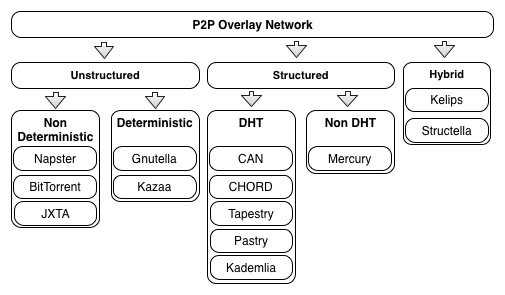
\includegraphics[width=0.75\textwidth]{./img/p2porganizations.jpg}
  \end{center}
  \caption{Different types of P2P Overlay networks organizations}
  \label{fig:Different types of P2P Overlay networks organizations}
\end{figure}


\paragraph{\textbf{Unstructured -}} % (fold)
\label{par:Unstructured}

We call `Unstructured' to a P2P system that doesn't require or define any constraint for the placement of data, these include Napster, Kazaa and Gnutella, famous for it's file sharing capabilities, where nodes can share their local files directly, without storing the file in any specific Node. There is however a `caveat' in the Unstructured networks, by not having an inherent way of indexing the data present in the network, performing a lookup results of the cost of asking several nodes the whereabouts of a specific file or chunk of the file, creating a huge performance impact with an increasing number of nodes. 

In order to calibrate the performance, Unstructured P2P networks offer several degrees of decentralization, one example is the evolution from Gnutella 0.4\cite{Definition2003} to Gnutella 0.6 \cite{T.Klingberg2002}\cite{Ripeanu2002a}, which added the concept of super nodes, entities responsible for storing the lookup tables for the files in parts of the network they are responsible for, increasing the performance, but adding centralized, single points of failure. 

Unstructured networks are classified\cite{Ranjan2006} in two types: deterministic and non-deterministic, defining that in a deterministic system, we can calculate before hand the number of hops needed to perform a lookup, knowing the predefined bounds, this includes systems such as Napster and BitTorrent\cite{Cohen2009}, in which the file transfers are decentralized, the object lookup remains centralized, keeping the data for the lookup tables stored in one place, which can be gathered by one of two ways: (i) peers inform directly the index server the files they have; or (ii) the index server performs a crawling in the network, just like a common web search engine, this gives this network a complexity of O(1) to perform a search, however systems like Gnutella 0.6, which added the super node concept, remain non deterministic because it's required to execute a query flood across all the super nodes to perform the search.

% paragraph Unstructured and Non-Deterministic (end)

\paragraph{\textbf{Structured with Distributed Hash Tables -}} % (fold)
\label{par:Structured with Distributed Hash Tables}

Structured P2P networks have an implicit way of allocating nodes for files and replicas storage, without the need of having any specie of centralized system for indexing, this is done by taking the properties of a cryptographic hash function \cite{Bakhtiari}\cite{Kargerl}\cite{Preneel1999}, such as SHA-1\cite{D.Eastlake3rdMotorola;P.JonesSystems2001}, which applies a transformation to any set of data with a uniform distribution of possibilities, creating an index with O(log(n)) peers, where the hash of the file represents the key and gives a reference to the position of the file in the network.

DHT's such as Chord\cite{Stoica2001}, Pastry\cite{Rowstron2001} and Tapestry\cite{Zhao2001}, use a similar strategy, mapping the nodes present in the network inside an hash ring, where each node becomes responsible for a segment of the hash ring, leveraging the responsibility to forward messages across the ring to his `fingers'(nodes that it knows the whereabouts). Kademlia\cite{Maymounkov} organizes it's nodes in a balanced binary tree, using XOR as a metric to perform the searches, while CAN\cite{Handley} introduced and a several dimension indexing system, in which a new node joining the network, will split the space with another node that has the most to leverage.

Evaluating the DHT Structured P2P networks raises identifiable issues, that result as the trade-off of not having an centralized infrastructure, responsible for railing new nodes or storing the meta-data, these are: (i) generation of unique node-ids is not easy achievable, we need always to verify that the node-id generated doesn't exist, in order to avoid collisions; (ii) the routing table is partitioned across the nodes, increasing the lookup time as it scales.

Table \ref{table:Complexity of structured P2P systems using a DHT}, showcases a comparison of the studied DHT algorithms.

\begin{table}
  \begin{tabular}{| p{1.3cm} | p{1.6cm} | p{1.9cm} | p{1.8cm} | p{1.6cm} | p{1.8cm} | p{1.8cm} |}
    \hline                        
    \textbf{P2P system} & \textbf{Overlay Structure} & \textbf{Lookup Protocol} & \textbf{Networking parameter} & \textbf{Routing table size} & \textbf{Routing complexity} & \textbf{Join/leave overhead} \\
    
    \hline
    Chord & 1 dimension, Hash ring & Matching key and NodeID & n= number of nodes in the network & O(log(n)) & O(log(n)) & O(log(n)\textsuperscript{2}) \\
    
    \hline
    Pastry & Plaxton style mesh structure & Matching key and prefix in NodeID & n= number of nodes in the network, b=base of identifier & O(log\textsubscript{b} (n)) & O(b log \textsubscript{b}(n)+b) & O(log(n)) \\
    
    \hline
    CAN & d-dimensional ID Space & Key value pair map to a point P in the D-dimensional space & n= number of nodes in the network, d=number of dimensions & O(2d) & O(d n\textsuperscript{1/2}) & O(2d) \\
    
    \hline
    Tapestry & Plaxton style mesh structure & Matching suffix in NodeID & n=number of nodes in the network, b=base of the identifier & O(log\textsubscript{b}(n)) & O(b log \textsubscript{b} (n)+b) & O(log(n)) \\
    
    \hline  
    Kademlia & Binary tree & XOR metric & n=number of nodes, m=number of different bits (prefix) & O(log(n)) & O(log\textsubscript{2}(n)) & not stable \\
    \hline      
  \end{tabular}
  \caption{Summary of complexity of structured P2P systems}
  \label{table:Complexity of structured P2P systems using a DHT}
\end{table}

% paragraph Structured with Distributed Hash Tables (end)

\paragraph{\textbf{Structured without Distributed Hash Tables -}} % (fold)
\label{par:Structured without Non-Distributed Hash Tables}

Mercury\cite{Bharambe}, a structured P2P network that uses a non DHT model, was designed to enable range queries over several attributes that data can be dimensioned on, which is desired on searches over keywords in several documents of text. Mercury design offers an explicit load balancing without the use of cryptographic hash functions, organizing the data in a circular way, named `attribute hubs'.

% paragraph Structured without Non-Distributed Hash Tables (end)

% \paragraph{\textbf{Hybrid -}} % (fold)
% \label{par:Hybrid}

% %TODO Structella , Kelips

% NOTE: Not sure if should include this, doesn't really include anything that new

% In recent developments, new generation P2P systems have evolved to combine both unstructured and structured P2P networks. We refer to this class of systems as hybrid. Structella [27] is one such P2P system that replaces the random graph model of an unstructured overlay (Gnutella) with a structured overlay, while still adopting the search and content placement mechanism of unstructured overlays to support complex queries. Other hybrid P2P design includes Kelips [60] and its variants. Nodes in Kelips overlay periodically gossip to discover new members of the network, and during this process nodes may also learn about other nodes as a result of lookup
% 12
% communication. Other variant of Kelips [56] allows routing table entries to store information for every other node in the system. However, this approach is based on assumption that system experiences low churn rate [70]. Gossiping and one-hop routing approach has been used for maintaining the routing overlay in the work [108]. In Table 4, we summarize the different P2P routing substrate that are utilized by the existing algorithms for organizing a GRIS.


% paragraph Hybrid (end)

\subsubsection{3.2.4 Fault Tolerance, Load Balancing, Assurance and Trust -}

Volunteer resource sharing means that we no longer have our computational infrastructure in a confined and well monitored place, this introducing new challenges that we have to address \cite{Koloniari2005} to maintain the system running with the minimum service quality, this issues can be: scalability, fault tolerance, persistence, availability and security\cite{Wallach} of the data and that the system doesn't get compromised. This part of the document serves to describe the techniques implemented in previous non centralized systems to address this issues.

\paragraph{\textbf{Fault Tolerance, Persistence and Availability}} % (fold)
\label{par:Fault Tolerance, Persistence and Availability}

are one of the key challenges in P2P community networks, due to it's churn uncertainty, making the system unable to assume the availability of Node storing a certain group of files. Previous P2P systems offer a Fault Tolerance and Persistence by creating file replicas, across several Nodes in the network, one example is PAST\cite{Druschel2001}\cite{Rowstron2001a}, a system that uses PASTRY routing algorithm, to determine which nodes are responsible to store a certain file, creating several different hashes which corresponds to different Nodes, guaranteeing an even distribution of files across all the nodes in the network. DynamoDB\cite{Decandia2007}, a database created by Amazon to provided an scalable NOSQL solution, uses a storage algorithm, inspired by the CHORD routing algorithm, in which stores file replicas in the consequent Nodes, in order to guarantee easy lookup if one of the Nodes goes down.

The strategy presented by the Authors of PAST to provide high availability, is an intelligent Node system, that use a probabilistic model, able to verify if there is an high request for a file, deciding to keep a copy and avoiding to overload the standard Node with every request that is made.

% paragraph Fault Tolerance, Persistence and Availability (end)

\paragraph{\textbf{Load Balancing}} % (fold)
\label{par:load_balancing}

in an optimal state, can be defined as having each node sharing roughly 1/N of the total load inside the network, if a Node has a significantly hight load compared with the optimal distribution, we call it a `heavy' node. There has been some research to find a optimal way to balance the load inside a P2P network, namely:

\begin{itemize}
   \item Power of Two Choices\cite{Byers} - Uses multiple hash functions to calculate different locations for an object, opts to store it in the least loaded node, where the other Nodes store a pointer. This approach is very simple, however it adds a lot of overhead when inserting data, however there is a proposed alternative of not using the pointers, which has the trade-off of increasing the message overhead at search.
   \item Virtual Servers\cite{Rao2003} - Presents the concept of virtualizing the Node entity to easy transfer it amongst the machines present in the P2P network. It uses two approaches, `one-to-one', where nodes contact other Nodes inside the network with the expectation of being able to trade some of the load, shifting a virtual server, or an `one-to-many/many-to-many' in which a directory of load per node is built, so that a node can make a query in order to find it's perfect match to distribute his load. Virtual Servers approach has the major issue of adding a extra amount of work to maintain the finger tables in each node.
   \item Thermal-Dissipation-based Approach\cite{Rieche} - Inspired by the heat expansion process, this algorithm shifts nodes position inside the hash ring windows of load responsibility, in a way that the load will implicitly flow from a node to it's close peers.
   \item Simple Address-Space and Item Balancing\cite{Karger2004} - It's an iteration over the virtual servers, by assigning several virtual nodes to each physical node, where only one of which is active at a time and this is only changed if having a different nodeId distribution in the network brings a more load balanced hash ring
 \end{itemize} 

S. Rieche, H. Niedermayer, S. Götz and  K. Wehrle from the University of Tübingen, made a study comparing this different approaches in a scenario using the CHORD routing algorithm, using a SHA-1 as the hashing function, with 4096 nodes and 100.000 to 1.000.000 documents and executing up to 25 runs per test, the results can be observed in the Figure ~\ref{fig:lbcomp}


\begin{figure}[htbp]
  \centering
  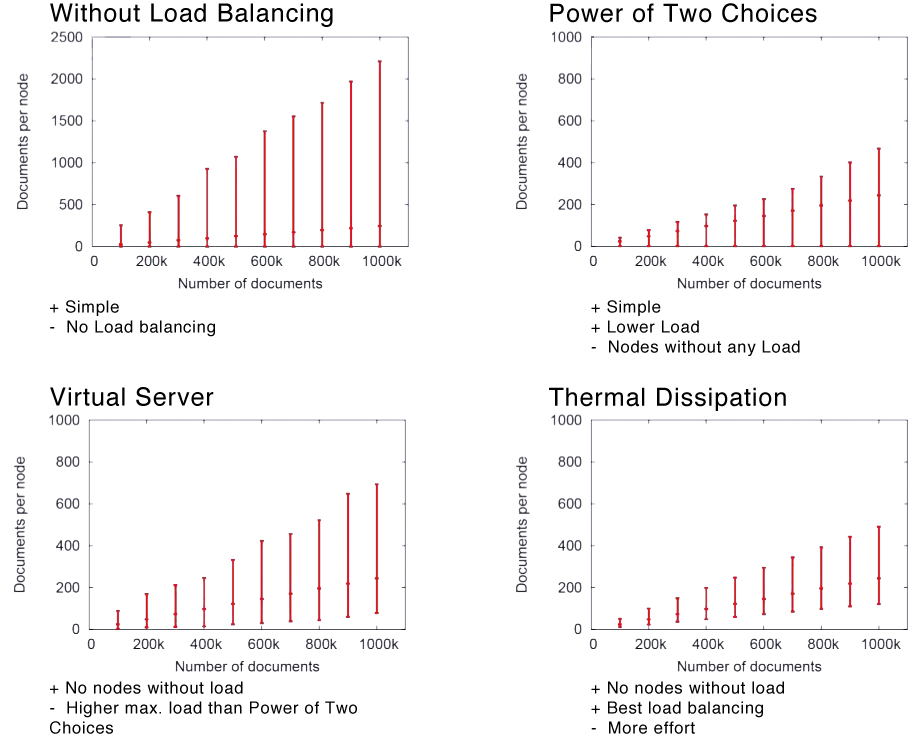
\includegraphics[width=1\textwidth]{img/lb.jpg}
  \caption{Load balancing approaches comparison}
  \label{fig:lbcomp}
\end{figure}


% paragraph load_balancing (end)

\paragraph{\textbf{Assurance and Trust}} % (fold)
\label{par:Assurance and Trust}

in a P2P network is an interesting challenge due to the lack of control over the machines that are willing to share with their resources, in order to achieve it, several strategies have been developed to maintain the integrity of the data using Cryptography, Reputation modeling schemes based on it's node previous record and also economic models, that resemble our own economy, but to share and trade computational resources.

Starting with the Cryptographic techniques, storage systems such as PAST give the option to the user to store encrypted content, disabling any other user, that does not have the encryption key, to have access to the content itself, this is a technique that comes from the Client-Server model, adapted to P2P environment, however, other cryptography technique benefits such as user authorization and identity, cannot be directly replicated into a P2P network without having a centralized authority to issue this validations, one of the alternatives is using distributed signature strategy, known as Threshold Cryptography \cite{Desmedt;1998}, where an access is granted if validated if several peers (a threshold), validates it's access, one implementation of Threshold Cryptography can be see in a P2P social network\cite{Afify} in order to guarantee privacy over the contents inside the network. 

Trust in a P2P system, as mentioned, is fundamental to it's well behaved functioning, not only in terms of data privacy, but also in giving the deserved resources to the executions that mostly need them, avoiding misbehaved peer intentions that can be a result of an Attack to jeopardize the network, one example is the known Sybil attack\cite{Douceura}. To achieve a fair trust sharing system, several metrics for a reputation mechanism have been developed \cite{Marti}, these can be seen in Table \ref{table:reputation}.

\begin{table}
  \centering
  \begin{tabular}{| c | c | c |}
    \hline                        
    \multicolumn{3}{|c|}{Reputation Systems} \\

    \hline                        
    Information Gathering & Scoring and Ranking & Response \\
    
    \hline                        
    Identity Scheme & Good vs. Bad Behavior & Incentives \\
    Info. Sources & Quantity vs. Quality & Punishment \\
    Info. Aggregation & Time-dependence &   \\ 
    Stranger Policy & Selection Threshold &   \\ 
      & Peer Selection &   \\ 

    \hline                           
  \end{tabular}
  \caption{Reputation system components and metric}
  \label{table:reputation}
\end{table}

Incentives for sharing resources\cite{Golle2001} can in the form of money rewards, greater speed access(used in Napster and some bittorrent networks) or it can be converted to a interchangeable rate to trade for more access to resources, giving the birth of economic models\cite{Filipe2011}\cite{Vishnumurthy}, that model the traded resources as a currency in which a peer has to trade in order to use the network.

% Economic Models
% * Gridlet Economics: Resource Management Models and Policies for Cycle-Sharing Systems
% * KARMA : A Secure Economic Framework for Peer-to-Peer Resource Sharing  (note: stores reputation remotly) Nead to Read


% paragraph Assurance and Trust (end)

% 
%---------{Resource sharing using the Web as platform}------------
% 
\subsection{Resource sharing using the Web platform} 

One of the main focuses with the proposed work, is to take advantage of the more recent developments of the Web platform to make the intended design viable (presented in section 4), the system depends on very lower level components such as:
\begin{itemize}
  \item High dynamic runtime for ongoing updates to the platform and specific assets for job execution
  \item Close-to-native performance for highly CPU-bound jobs
  \item Peer-to-peer interconnectivity
  \item Scalable storage and fast indexing
\end{itemize}

Therefore, we present in this section the relevant components present or undergoing a development process for the Web platform, such as: Javascript, Emscripten, IndexedDB, WebRTC and HTTP2.0. These will coexist as key enablers for  the necessary features to such a distributed shared resource system:

\subsubsection{3.3.1 Web Platform}

Since the introduction of AJAX\cite{Google/Mozzila/Opera}, the web has evolved into a new paradigm where it left being a place of static pages, known as Web 1.0. Nowadays, we can have rich web applications with degrees of interaction and levels of performance close to a native application. The programming languages that power the Web Platform, in special HTML, CSS and JavaScript\cite{Ecma2009}, have been subject to several changes, enabling `realtime' data transfers and fluid navigations through content. Javascript, an interpreted language with an high dynamic runtime, has proven to be the right candidate for a modular Web Platform, enabling applications to evolve continuously over time, by simply changing the pieces that were updated.

\textbf{Emscripten}\cite{Zakai2011}, a LLVM(Low Level Virtual Machine) to JavaScript compiler, enabled native performance on Web apps by compiling any language that can be converted to LLVM bytecode, for example C/C++, into JavaScript. This tool enabled native game speed on the browser, where two of the major examples are the project Codename: ``BananaBread''\footnote{Mozilla, BananaBread,  URL: https://developer.mozilla.org/en/demos/detail/bananabread, seen in December 2013} and ``Epic Citadel''\footnote{Mozilla, Epic Citadel,  URL: http://www.unrealengine.com/html5/, seen in December 2013}, in which Mozilla used Ecmascripten to port the entire Unreal Engine 3 to JavaScript. In Figure~\ref{fig:dan}, we can see a comparison of the performance of several algorithms, running on Dalvik, Android Java runtime, asm.js, the subset of Javascript that the code in C/C++ is transformed into when compiled with Emscripten and Native, the same C/C++ but running on a native environment. The results are very interesting, specially in the first test, where asm.js outperforms native. The explanation for this is due to the fact that BinaryTrees use a significant amount of `malloc' invocations, which is an expensive system call, where in asm.js, the code uses typed arrays, using `machine memory', which is flat allocated in the beginning of the execution for the entire run.

\begin{figure}[h!]
  \centering
  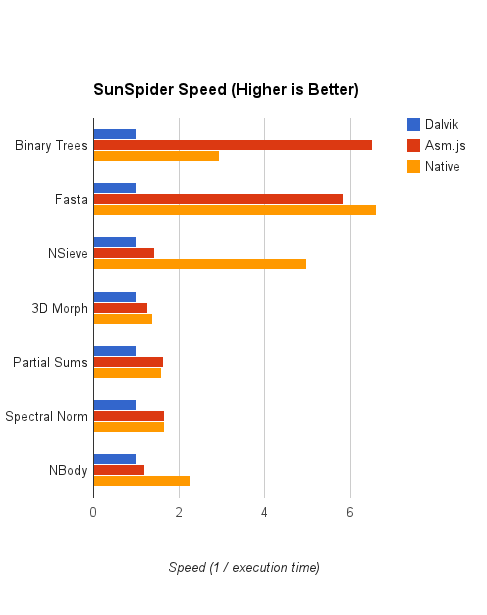
\includegraphics[width=0.82\textwidth]{img/Dalvik-vs-ASM-vs-Native-edited}
  \caption{Dalvik vs. ASM.js vs. Native performance}
  \label{fig:dan}
\end{figure}

\textbf{WebRTC}\cite{IanHickson2013}, a technology being developed by Google, Mozilla and Opera, with the goal of enabling Real-Time Communications in the browser via a JavaScript API. WebRTC brings to the browser the possibility of peer-to-peer interoperability. Peers perform their handshake through a `Signaling Server'. The signaling server will exchange the `ICE(Interactive Connectivity Establishment) candidates' of each peer as this serves as an invite so a data-channel can be opened, a visualization of this process can be seen in Figure~\ref{fig:webrtc}. Since most of the browsers sit behind NAT, there is another server, named `Turn'(Relay), which tells to each browser their public IP in the network. WebRTC, although being built with the goal of real-time voice and video communications, has also been shown as a viable technology do distribute content, as seen in PeerCDN and SwarmCDN\cite{Vogt}.

\begin{figure}[h!]
  \centering
  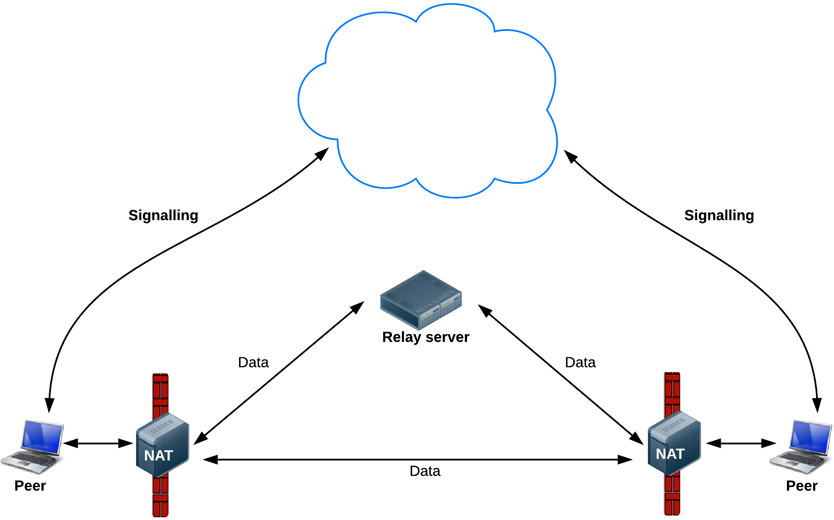
\includegraphics[width=0.95\textwidth]{img/webrtc.png}
  \caption{Example of a WebRTC session initiation}
  \label{fig:webrtc}
\end{figure}

% 
% There is also Jingle
% https://github.com/legastero/jingle.js
% Jingle is an extension of XMPP that enables P2P and communication over RTC
% 


\textbf{`level.js'} offers an efficient way to store larger amounts of data in the browser machine persistent storage, its implementation works as an abstraction on top of the leveldown API on top of IndexedDB\cite{Recommendation2013}, which in turn is implemented on top of the LevelDB\cite{JeffreyDean;SanjayGhemawat}, an open source on-disk key-value store inspired by Google BigTable. IndexedDB is an API for client-side storage of significant amounts of structured data and for high performance searches on this data using indexes. Since `level.js' runs on the browser, we have an efficient way to storage data and quickly retrieve it.

One of the latest improvements being built for the Web Platform is the new HTTP spec, \textbf{HTTP2.0}\cite{Thomson2013}, this next standard after HTTP1.1 which aims to improve performance towards a more realtime oriented web, while being retrocompatible at the same time. Several advancements in this new spec are:

\begin{itemize}
  \item Parallel requests - HTTP1.1 was limited by a max of 6 parallel requests per origin and taking into account that the mean number of assets is around one hundred when loading an webapp, it means that transfers get queued and slowed down. In order to overcome this, we could distribute the assets through several origins in order to increase the throughput. However this optimization backfired when in mobile, since there was a lot of signaling traffic in TCP layer, starving the user connection. HTTP2.0 no longer has this constraint.
  \item Diff updates - One of the web developer favorites has been concatenating their javascript files so the response payload decreases, however, in modern webapps, most of the time, we do not want the user to download the entire webapp again, but only some lines of code referring to the latest update. With diff updates, the browser will only receive what has been changed.
  \item Prioritization and flow control - Different webapp assets have different weights in terms of user experience, with HTTP2.0, the developer can set priorities so the assets arrive by order.  A simple flow control example can be seen on Figure~\ref{fig:http2dataflow}, where the headers of the file gain priority as soon as they are ready, and get transfered immediately. 
  \item Binary framing - In HTTP2.0, binary framing is introduced with the goal of creating more performant HTTP parsers and encapsulating different frames as seen on Figure~\ref{fig:binaryframing}, so they can be send in an independent way.
  \item HTTP headers compression - HTTP2.0 introduces an optimization with headers compression\cite{Ruellan2013} that can go to a minimum of 8 bytes in identical requests, against the 800 bytes in HTTP1.1. This is possible because of the state of the connection is maintained, so if a identical requests is made, changing just one of the resources (for example path:/user/a to path:/user/b), the client only has to send that change in the request.
  \item Retrocompatibility - HTTP2.0 respects the common headers defined by HTTP1.1, it doesn't include any change in the semantics.
\end{itemize}

\begin{figure}[htbp]
  \centering
  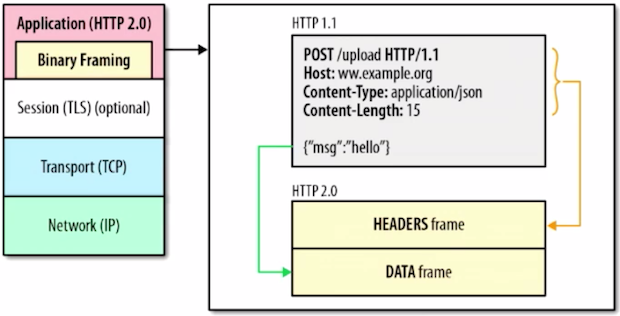
\includegraphics[width=0.95\textwidth]{img/http2binaryframing.png}
  \caption{HTTP2.0 Binary framing}
  \label{fig:binaryframing}
\end{figure}

\begin{figure}[htbp]
  \centering
  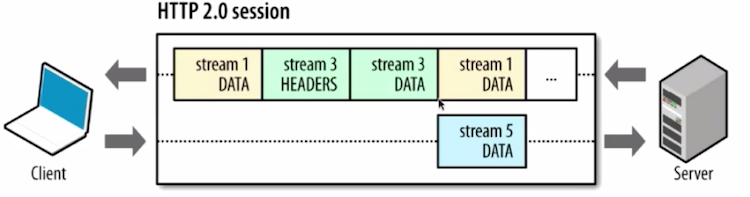
\includegraphics[width=0.95\textwidth]{img/http2dataflow.png}
  \caption{Example of an HTTP2.0 dataflow}
  \label{fig:http2dataflow}
\end{figure}


\subsubsection{3.3.2 Previous attempts on cycle sharing through web platform}
The first research of browser-based distributed cycle sharing was performed by Juan-J. Merelo, et. al., which introduced a Distributed Computation on Ruby on Rails framework\cite{Merelo2007}. The system used a client-server architecture in which clients, using a browser would connect to a endpoint, where they would download the jobs to be executed and sent back the results. In order to increase the performance of this system, a new system\cite{Duda2013} of browser-based distributed cycle sharing was creating using Node.js as a backend for very intensive Input/Output operations\cite{Tilkov2010}, with the goal of increased efficiency, this new system uses normal webpages(blogs, news sites, social networks) to host the client code that will connect with the backend in order to retrieve and execute the jobs, while the user is using the webpage, this concept is known as parasitic computing\cite{Barabasi2001}, where the user gets to contribute with his resources without having to know exactly how, however since it's Javascript code running on the client, any user has access to what is being processed and evaluate if it presents any risk to the machine.


\subsection{Analysis and discussion}

 % ISTO É pARA FAZER UM SUM UP